\section{Transport: the closed loop under uniform translation}
\label{sec:tpf}

This section measures the closed loop: the face fractions set the normal, the normal sets the clipping surface, and the clipping surface sets the next face fractions. Two loops were built in a fork of the TwoPhaseFlow library of \citet{ScheuflerRoenby2023TwoPhaseFlow}, inside the isoAdvector--plicRDF framework \citep{RoenbyEtAl2016,ScheuflerRoenby2019} that the comparators use: the plane-clipped loop, in which the clipping surface is the PLIC plane positioned by $\alpha_k$ and the volume fluxes are isoAdvector's, and the dual advection with one surface per cell, in which a paraboloid serves the volume flux and the face update alike. Both are measured on a translated plane and on a translated sphere. The results are stated here with the tables and figures that carry the numbers; the implementation record of every measurement, in the same order, is \ref{app:transport}.

\subsection{Setup}
\label{sec:tpf-setup}

The state is initialised by the constructions of \cref{sec:static}. In the plane-clipped loop a reconstruction scheme forms the normal \cref{eq:avof-normal} from the stored face fractions and positions the PLIC plane by $\alpha_k$ with the library's bisection; isoAdvector sweeps every face of an interface cell with the moving plane, the submerged area of the face at the end of the step is the new face fraction, and a face shared by two interface cells takes the upwind cell's plane, consistent with its volume flux. By \cref{eq:clipping-law} this plane clipping gives first-order face fractions, $q = 1$; it is measured first on purpose, as the baseline for the paraboloid. The time step is fixed at a Courant number $\mathrm{Co} = |\mathbf{U}|\Delta t/h$; a run is recorded as diverged when $\alpha$ leaves $[-0.5, 1.5]$ or the number of interface cells exceeds ten times its initial value. The translated plane is the plane of \cref{sec:plane}, carried over $0.2L$ along its normal and along $(1, 0, 0)$, $N = 20$ to $160$; the translated sphere has $R = 0.15$ in a $2 \times 1 \times 1$ box and is carried by $\mathbf{U} = (1, 0, 0)$ over one box length, 3.3 diameters, $N = 32$, $64$, $128$ cells across the box height ($R/h = 4.8$ to $19$). \Cref{tab:tpf-sources} lists the normal sources that drive the loop and the controls. Every prediction was pre-registered in the study configuration before the run; the ones that failed are reported where they failed.

\begin{table}[htbp]
\centering
\caption{The normal sources of the closed loop, the controls and the comparators. Every row runs on the identical initial state; plicRDF and isoAlpha run on the same $\alpha_k$ (the Detrixhe--Aslam cell fraction, not the one their own initialisation would give).}
\label{tab:tpf-sources}
\footnotesize
\begin{tabular}{p{0.26\linewidth}p{0.66\linewidth}}
\toprule
normal in the loop & definition \\
\midrule
own normal & \cref{eq:avof-normal} on the cell's own faces, as it stands \\
ring normal & \cref{eq:avof-normal} on the union of the cell's ring: $\mathbf{n}_k = \sum_j \mathbf{m}_j / |\sum_j \mathbf{m}_j|$ over the point neighbours $j$ (the interior faces cancel); exact for a plane, never divided by a small area, the mean normal of the patch \\
ring quadric & the normal at the cell of a weighted least-squares Monge patch through the ring's recovered planes (\cref{sec:curv}) \\
exact normal (control) & the normal of the translated surface; the loop is open \\
plicRDF normal (control) & the plicRDF normal from $\alpha_k$ in the DAVOF update \\
\midrule
plicRDF, isoAlpha & the library's own methods on the same $\alpha_k$; they carry no face fractions \\
\bottomrule
\end{tabular}
\end{table}

\subsection{Why the cell's own normal cannot drive the loop}
\label{sec:tpf-sliver}

In the loop each face takes its fraction from the surface of its upwind cell, so the fractions of one cell come from several surfaces, which agree only in exact arithmetic. Linearised about the exact plane, the turn of the cell's area vector $\mathbf{m}_k$ is the neighbours' displacement at the traces of the faces they set, weighted by the trace length times its lever arm of about $h/2$, divided by the cell's own patch area $A$. The own faces' weights sum to one, so the loop has no restoring force, and a foreign weight exceeds one where $A$ is small against the lever arm: in a sliver cell, an interface cell whose wetted area is a small fraction of $h^2$. The stencil reconstructions of classical VOF average the volume fractions of a neighbourhood before anything is divided and never meet this. Sliver cells are not rare (\cref{tab:tpf-sliver}); a rule that treats them specially acts on about one cell in eight at every resolution. Measured cell by cell on one plane run at $N = 80$, the linearised sum predicts the turn (correlation $0.99$, median ratio $1.0$), cells fed only their own surface turn by their own tilt, and the loop grows as one mode. The own-normal runs start at round-off and grow geometrically from the second step, by $1.10$ to $1.26$ per step at $\mathrm{Co} = 0.2$ and $1.6$ to $8.8$ at $0.5$: the linear instability of an exact fixed point, independent of the clipping surface. The ring normal divides the same mismatch by about $9h^2$ and contracts, at the price of being the mean normal of a patch of width $3h$.

\begin{table}[htbp]
\centering
\caption{Sliver cells on the translated sphere: the share of interface cells with $|A_{\tilde\Sigma_k}| < 0.1 h^2$ at the first step and over a run.}
\label{tab:tpf-sliver}
\footnotesize
\begin{tabular}{lrrr}
\toprule
 & $N = 32$ & $N = 64$ & $N = 128$ \\
\midrule
first step & $11.5\,\%$ & $13.6\,\%$ & $11.3\,\%$ \\
over a run & \multicolumn{3}{c}{$8$ to $14\,\%$} \\
\bottomrule
\end{tabular}
\end{table}

\subsection{The plane-clipped loop}
\label{sec:tpf-plane-loop}

\Cref{tab:tpf-plane} scores the translated plane, \cref{tab:tpf-sphere} the translated sphere, \cref{fig:tpf-history} the error against the step. On the plane the ring normal, the ring quadric and the exact normal keep the face fractions and the normal at round-off in all 32 runs each; the own normal breaks at $N = 160$ and at $\mathrm{Co} = 0.5$ from $N = 40$ on, and the plicRDF normal fails the gate everywhere, because it is not exact on the corner cells of a plane. On the sphere the ring normal is the first stable DAVOF transport loop: bounded to $10^{-14}$ and conservative to round-off at every resolution and Courant number, where the own normal is stopped after 45 to 232 steps and the ring quadric stays bounded but erratic, its fit failing in up to 1700 cells per step. The face fractions transport at first order with the ring normal and with the exact normal alike: the order is the plane clipping's, $q = 1$ by \cref{eq:clipping-law}, not the normal's. Against plicRDF on the same $\alpha_k$ the ring normal is first order at $1.1$ to $1.35$ times plicRDF's error, the centroid is second order at plicRDF's value to three digits, the shape error is plicRDF's, and the cost is below plicRDF's (\cref{tab:tpf-cost}). At fixed $N$ the ring normal's errors rise as the Courant number falls (\cref{tab:tpf-courant}), because the per-step clipping error accumulates over the $1/\mathrm{Co}$ times more steps; the pre-registered prediction of the opposite direction was falsified. One result is open: the loop driven by the plicRDF normal does not converge on the sphere, although plicRDF alone converges on the same $\alpha_k$ (\ref{app:transport}).

\begin{table}[htbp]
\centering
\caption{The translated plane in TwoPhaseFlow: the plane of \cref{sec:plane} carried over $0.2L$ along its normal and along $(1, 0, 0)$, $N = 20, 40, 80, 160$, $\mathrm{Co} = 0.05$ to $0.5$. For every normal source and Courant number the number of the eight runs (two directions, four meshes) in which the face fractions and the normal stay at round-off over the whole run (both run maxima of $L_1$ below $10^{-12}$); the last column is the run maximum of $L_1(\alpha_f)$ at $N = 160$ and $\mathrm{Co} = 0.5$ on the normal arm (for plicRDF and isoAlpha, which carry no face fractions, the normal error). Table body generated by \texttt{make\_table\_advection.py} from the study table.}
\label{tab:tpf-plane}
\footnotesize
\setlength{\tabcolsep}{4pt}
\resizebox{\linewidth}{!}{% written by prepare_tables.py from table_advection_plane.tex -- do not edit
% Auto-generated by docs/davof/davof-article/make_table_advection.py -- do not edit.
\begin{tabular}{lrrrrr}
\toprule
normal & Co $= 0.05$ & Co $= 0.1$ & Co $= 0.2$ & Co $= 0.5$ & $\max_t L_1(\alpha_f)$, $N = 160$, Co $= 0.5$ \\
\midrule
DAVOF, ring normal & 8/8 & 8/8 & 8/8 & 8/8 & 6.24e-14 \\
DAVOF, own normal & 4/8 & 4/8 & 1/8 & 1/8 & 3.64e-01 \\
DAVOF, exact normal (control) & 8/8 & 8/8 & 8/8 & 8/8 & 5.48e-14 \\
DAVOF, plicRDF normal & 0/8 & 0/8 & 0/8 & 0/8 & 9.89e-02 \\
DAVOF, ring quadric & 8/8 & 8/8 & 8/8 & 8/8 & 5.72e-14 \\
plicRDF & -- & -- & -- & -- & 7.07e-02 (normal) \\
isoAlpha & -- & -- & -- & -- & 1.76e-01 (normal) \\
\bottomrule
\end{tabular}
}
\end{table}

\begin{table}[htbp]
\centering
\caption{The translated sphere in TwoPhaseFlow: $R = 0.15$ in a $2 \times 1 \times 1$ box carried by $\mathbf{U} = (1, 0, 0)$ over one box length, 3.3 diameters, $N = 32, 64, 128$ cells across the box height ($R/h = 4.8$ to $19$), $\mathrm{Co} = 0.1, 0.2, 0.5$. Errors at the end of the run on the finest mesh and the least-squares order $p$ over the three meshes: $L_1(\alpha_f)$ the face-fraction error as a fraction over the faces of the interface cells, $L_1(\mathbf{n})$ and $L_1(\mathbf{x})$ the normal and centroid errors of the recovered planes against the translated sphere, $E_{\mathrm{shape}}$ the volume of the symmetric difference between the transported and the exact liquid. The own normal aborts at the listed steps (interface cells above ten times the initial count) for $N = 32/64/128$. Every other run is bounded to $10^{-14}$ and conservative to round-off. Table body generated by \texttt{make\_table\_advection.py}.}
\label{tab:tpf-sphere}
\footnotesize
\setlength{\tabcolsep}{3.5pt}
\resizebox{\linewidth}{!}{% written by prepare_tables.py from table_advection_sphere.tex -- do not edit
% Auto-generated by docs/davof/davof-article/make_table_advection.py -- do not edit.
\begin{tabular}{llrrrrrrr}
\toprule
normal & Co & $L_1(\alpha_f)$ & $p$ & $L_1(\mathbf{n})$ & $p$ & $L_1(\mathbf{x})$ & $p$ & $E_{\mathrm{shape}}$ \\
\midrule
DAVOF, ring normal & 0.1 & 7.72e-03 & 0.80 & 1.26e-02 & 0.94 & \textbf{1.34e-04} & 1.86 & \textbf{3.90e-05} \\
 & 0.2 & 5.76e-03 & 0.81 & 1.09e-02 & 0.95 & \textbf{1.02e-04} & 1.86 & \textbf{3.05e-05} \\
 & 0.5 & 2.96e-03 & 1.00 & 8.12e-03 & \textbf{1.02} & 4.88e-05 & 1.99 & \textbf{1.58e-05} \\
\midrule
DAVOF, own normal & 0.1 & \multicolumn{7}{l}{aborted at step 205/232/177} \\
 & 0.2 & \multicolumn{7}{l}{aborted at step 111/117/97} \\
 & 0.5 & \multicolumn{7}{l}{aborted at step 46/56/45} \\
\midrule
DAVOF, exact normal (control) & 0.1 & 3.84e-03 & 0.85 & \textbf{5.55e-04} & \textbf{1.43} & \textbf{7.93e-05} & \textbf{1.92} & \textbf{2.19e-05} \\
 & 0.2 & 3.32e-03 & 0.82 & \textbf{4.70e-04} & \textbf{1.48} & \textbf{6.76e-05} & 1.93 & \textbf{1.94e-05} \\
 & 0.5 & 3.46e-03 & 0.99 & \textbf{5.54e-04} & \textbf{1.90} & \textbf{4.76e-05} & 1.98 & \textbf{1.58e-05} \\
\midrule
DAVOF, plicRDF normal & 0.1 & 2.19e-02 & 0.16 & 5.17e-02 & 0.05 & 5.11e-04 & 1.03 & 6.75e-05 \\
 & 0.2 & 1.68e-02 & 0.15 & 4.10e-02 & -0.01 & 3.09e-04 & 1.18 & 6.26e-05 \\
 & 0.5 & 8.57e-03 & 0.24 & 2.70e-02 & -0.11 & 1.33e-04 & 1.26 & 3.40e-05 \\
\midrule
\midrule
DAVOF, ring quadric & 0.1 & 7.97e-03 & 0.82 & \textbf{7.80e-03} & \textbf{1.09} & \textbf{1.39e-04} & 1.88 & 3.98e-05 \\
 & 0.2 & 6.02e-03 & 1.86 & \textbf{5.49e-03} & \textbf{2.61} & 1.05e-04 & \textbf{3.49} & 3.10e-05 \\
 & 0.5 & 3.38e-03 & 1.06 & \textbf{1.50e-03} & \textbf{1.60} & \textbf{4.71e-05} & 1.98 & \textbf{1.57e-05} \\
\midrule
\midrule
\midrule
\midrule
\midrule
plicRDF & 0.1 & -- & -- & 1.14e-02 & 1.03 & 1.40e-04 & 1.90 & 3.93e-05 \\
 & 0.2 & -- & -- & 9.20e-03 & 1.04 & 1.04e-04 & 1.94 & 3.08e-05 \\
 & 0.5 & -- & -- & 6.03e-03 & 0.97 & 4.87e-05 & 1.99 & 1.61e-05 \\
\midrule
isoAlpha & 0.1 & -- & -- & 2.29e-02 & 0.80 & 1.62e-04 & 1.87 & 4.58e-05 \\
 & 0.2 & -- & -- & 2.03e-02 & 0.74 & 1.20e-04 & 1.87 & 3.53e-05 \\
 & 0.5 & -- & -- & 1.65e-02 & 0.64 & 5.97e-05 & 1.85 & 1.71e-05 \\
\bottomrule
\end{tabular}
}
\end{table}

\begin{figure}[htbp]
\centering
\includegraphics[width=0.78\linewidth]{{davof_advection_history_sphereTranslation3D_hex_N64_Co0.2}.png}
\caption{The face-fraction error $L_1(\alpha_f)$ against the step for the translated sphere at $N = 64$ and $\mathrm{Co} = 0.2$ (320 steps), plane-clipped loop. The own normal grows from the first steps and is stopped at step 117; the ring normal and the ring quadric grow slowly from the $O(h/R)$ clipping error of the first step; the exact-normal control saturates; the plicRDF-normal control grows as the ring normal does at a higher level.}
\label{fig:tpf-history}
\end{figure}

\begin{table}[htbp]
\centering
\caption{The Courant dependence at fixed resolution. Plane-clipped loop with the ring normal at $N = 64$: the error accumulates over the $1/\mathrm{Co}$ steps and rises as the Courant number falls. Dual advection with the ring-tensor paraboloid and the ring normal at $N = 128$: the error no longer accumulates and rises with the pre-image's displacement, i.e.\ with the Courant number. The exact-normal controls are flat in the Courant number in both loops.}
\label{tab:tpf-courant}
\footnotesize
\begin{tabular}{llrrr}
\toprule
loop & error & $\mathrm{Co} = 0.1$ & $\mathrm{Co} = 0.2$ & $\mathrm{Co} = 0.5$ \\
\midrule
plane-clipped, ring normal, $N = 64$ & $L_1(\alpha_f)$ & 1.22e-02 & 9.45e-03 & 6.06e-03 \\
 & $L_1(\mathbf{n})$ & 2.53e-02 & 2.23e-02 & 1.84e-02 \\
paraboloid by volume, ring normal, $N = 128$ & $L_1(\alpha_f)$ & 8.52e-04 & 8.71e-04 & 1.22e-03 \\
\bottomrule
\end{tabular}
\end{table}

\subsection{A second-order clipping inside the plane loop does not repair it}
\label{sec:tpf-sagitta}

The plane is $O(h^2)$ off the interface, so the leading-order repair that stays within the plane loop corrects the clipped area of every face by the sagitta between the interface's arc and the plane's chord on the face, from the ring curvature tensor of \cref{sec:curv} (the formula is in \ref{app:transport}). \Cref{tab:tpf-sagitta} shows what it does: in pure geometry it removes nearly all of the plane's face error; after one step from the exact state it removes $93\,\%$; over a run it keeps $27$ to $30\,\%$ of that gain and leaves the order at one; on the chord-initialised state it doubles the error from the first step. The per-face fields locate the cause in the volume anchor: the volume fluxes are the volumes under the moving plane, so within the $1/\mathrm{Co}$ steps in which a cell holds the interface $\alpha_k$ acquires a one-signed $O(h/R)$ deviation from the volume under the surface, and a correction that is right for the exact state overshoots. This is the finding of \cref{sec:regen} under transport: a volume anchor is consistent only in the quadrature that defined the cell fraction. The requirement that follows is measured, not assumed: the volume flux and the face update must be the volume and the boundary moments of one surface per cell.

\begin{table}[htbp]
\centering
\caption{The sagitta correction of the plane-clipped face areas (\texttt{faceClipping planeSagitta} of the fork), translated sphere, exact normal in the loop, $\mathrm{Co} = 0.2$ unless stated. The DA-Q state keeps the chord cell fraction of the Detrixhe--Aslam construction; the exact state has $\alpha_k$ equal to the volume under the sphere. Orders over $N = 32$, $64$, $128$.}
\label{tab:tpf-sagitta}
\footnotesize
\begin{tabular}{p{0.36\linewidth}p{0.28\linewidth}p{0.28\linewidth}}
\toprule
test & plane clipping & with the correction \\
\midrule
pure geometry: random cubes cut by a sphere, exact tensor and volume, $h/R = 0.21$ to $0.05$ & -- & $92$ to $97\,\%$ of the plane's face error removed \\
one step, exact state, $N = 32$, $\mathrm{Co} = 0.02$ & $L_1(\alpha_f) = 6.34\cdot10^{-3}$ & $4.40\cdot10^{-4}$ ($93\,\%$ removed; $90\,\%$ at $\mathrm{Co} = 0.2$) \\
one step, DA-Q state, $N = 32$ & $2.78\cdot10^{-3}$ & $6.22\cdot10^{-3}$ \\
run, DA-Q state, $N = 32/64/128$ & $1.04\cdot10^{-2}$, $5.68\cdot10^{-3}$, $3.32\cdot10^{-3}$ (order $0.82$) & $1.03\cdot10^{-2}$, $5.53\cdot10^{-3}$, $3.23\cdot10^{-3}$ ($0.83$) \\
run, exact state, $N = 32/64/128$ & $1.15\cdot10^{-2}$, $6.24\cdot10^{-3}$, $3.64\cdot10^{-3}$ & $8.42\cdot10^{-3}$, $4.33\cdot10^{-3}$, $2.58\cdot10^{-3}$ ($0.85$); $27$ to $30\,\%$ of the one-step gain kept \\
\bottomrule
\end{tabular}
\end{table}

\subsection{One surface per cell: the dual advection}
\label{sec:tpf-dual}

One time step of the dual advection: (1) the normal and the position of every interface cell follow from $(\alpha_k, \{\alpha_f\})$ by \cref{eq:avof-normal,eq:avof-position}; (2) the curvature tensor of the cell is taken from the ring of recovered normals (\cref{sec:curv}); (3) a surface is built in the frame of the normal; (4) $\alpha_k$ is advanced by the liquid volume of the prism swept between each face's pre-image $f - \mathbf{U}\Delta t$ and the face under the surface of the upwind cell; (5) each $\alpha_f$ is advanced by the pre-image's liquid fraction under the same surface. The surface is a quadric, so along any segment it is a quadratic polynomial with exact roots, and the pre-image cut is the exact face cut of \cref{sec:static} up to its Gauss rule. A face shared by two interface cells takes the upwind cell's surface; a face whose two cells carry no surface takes the closest neighbouring one. Three surfaces were run on the translated sphere at $N = 32$ and $\mathrm{Co} = 0.2$ over 160 steps (\cref{tab:tpf-surfaces}). The exact sphere as every cell's surface is the gate of the machinery, not a test of the method, and it holds: the update reproduces the exact state to round-off and transports an inconsistent initial state unchanged. The six-coefficient surface of \cref{sec:full}, which interpolates the cell's own face fractions, is unstable: the faces of a cell come from different surfaces, so the six fractions are not the fractions of any one paraboloid, and a surface that interpolates them carries their inconsistency to the next pre-images amplified; the zero-velocity map is the identity on this surface, a neutral fixed point, and the displaced pre-images push it past one. The surface that is stable takes nothing from the cell's own faces beyond the normal: the frame of the normal, the curvature tensor of the ring, zero slopes, and the offset from the conserved $\alpha_k$ as in classical VOF, with a second-order surface in place of the plane and with the surface's own volume flux. The plane loop is stable with the ring normal for the same reason: its one degree of freedom beyond the normal, the position, comes from $\alpha_k$. The volume anchor, the quadrature and volume rules and the parallel exchange are described in \ref{app:transport}.

\begin{table}[htbp]
\centering
\caption{The three surfaces of the dual advection on the translated sphere, $N = 32$, $\mathrm{Co} = 0.2$, 160 steps, exact-sphere initial state, split quadrature for the volumes (\ref{app:transport}). Errors at the end of the run; the plane-clipped loop on the same state in parentheses.}
\label{tab:tpf-surfaces}
\footnotesize
\begin{tabular}{p{0.30\linewidth}p{0.17\linewidth}p{0.45\linewidth}}
\toprule
surface & normal in the frame & outcome \\
\midrule
exact sphere (gate) & -- & face fractions exact to $10^{-14}$ from the second step on; $\alpha$ bounded to $10^{-17}$, conservative to $3\cdot10^{-17}$; the chord deficit of a DA-Q initial state ($8\cdot10^{-3}$ of $V$) is transported unchanged \\
\midrule
six-coefficient paraboloid fitted to the cell's own face fractions (\cref{sec:full}) & exact / own / ring & first step better than the plane loop's by $20$ / $13$ / $2.6$ ($2.2\cdot10^{-4}$ against $4.4\cdot10^{-3}$ with the exact normal); then the error grows by $2$ to $2.5$ per step and the run is stopped at step 10 to 21, with every normal, at $\mathrm{Co} = 0.05$ as at $0.2$, at both quadrature tolerances; a volume shift of the offset after the fit changes nothing; the one-scalar face anchoring of \cref{sec:regen} is stopped at step 81 \\
\midrule
ring-tensor paraboloid positioned by $\alpha_k$ & exact & bounded to $10^{-20}$, conservative, surface defect at the anchor's tolerance; $L_1(\alpha_f) = 5.7\cdot10^{-4}$ ($1.15\cdot10^{-2}$); normal from the cell's own faces $2.8\cdot10^{-4}$ ($3.7\cdot10^{-3}$); centroid $4.1\cdot10^{-4}$ ($7.7\cdot10^{-4}$); maximum face error $2.4\cdot10^{-2}$ on a few grazing cells \\
 & ring & $L_1(\alpha_f) = 5.9\cdot10^{-3}$ ($1.78\cdot10^{-2}$); centroid $5.3\cdot10^{-4}$ ($1.35\cdot10^{-3}$); transported normal $3.3\cdot10^{-2}$, the ring normal's own bias \\
 & own & diverges through the sliver cells, as the plane loop does \\
\bottomrule
\end{tabular}
\end{table}

\subsection{The resolution ladder}
\label{sec:tpf-ladder}

The ring-tensor paraboloid positioned by $\alpha_k$ was run over the resolutions and Courant numbers of \cref{tab:tpf-sphere} from the exact-sphere initial state, with the volume rule of \citet{KromerBothe2023Init}, and on the translated plane of \cref{tab:tpf-plane}. \Cref{fig:tpf-ladders} plots the ladders against the plane-clipped loop, \cref{tab:tpf-curved} carries the numbers, \cref{tab:tpf-curved-plane} the plane gate. Three results. First, the order of the closed loop is the order of the normal fed back: the face fractions are of order $2.84$ per period with the exact normal, $2.11$ with the ring quadric's normal and $1.35$ with the ring's mean normal, and the orders after the first step ($2.76$, $1.92$, $1.05$) are the same. The error at the end of the run is a constant factor of $1.8$ to $2.0$ above the error after the first step: the per-step remainder does not accumulate over the period, which answers the question of \cref{sec:transport} in the negative. Second, every row is bounded and conservative at every resolution and Courant number, the volume anchor converges in every cell, and on the plane the exact and the ring normal hold the gate in all 16 runs each; the own normal diverges at every resolution and Courant number, and the variant that keeps the own normal above the sliver threshold diverges in eight of nine runs (its pre-registered prediction was falsified): the whole loop needs the filtered normal. Third, the fourth mesh settles the asymptotic order of the computed normals (\cref{tab:tpf-n256}): from $N = 128$ to $256$ the ring quadric's row is of order $1.17$ in the face fractions and $1.18$ in the normal, the ring mean's $1.16$ and $1.04$, the exact normal's $2.30$; a fit $c_1 h + c_2 h^2$ through the two finest meshes puts $88\,\%$ of the ring quadric's error at $N = 256$ in the first-order term, and the ratio of the two computed-normal rows is constant ($18.4$ and $18.6$). The computed-normal loop is therefore first order asymptotically, with the ring quadric's normal buying a constant eighteen times smaller than the ring mean's, not an order; second order over a period is reached only in the frame of the exact normal. With the ring quadric's normal the transported normal at $N = 128$ is fifty times below the ring normal's and plicRDF's, the fit converges in every interface cell of every step, and the row's four pre-registered predictions held, the normal's order at the margin. The Courant dependence has reversed against the plane loop (\cref{tab:tpf-courant}): the error no longer accumulates over the steps and rises with the pre-image's displacement.

\begin{figure}[htbp]
\centering
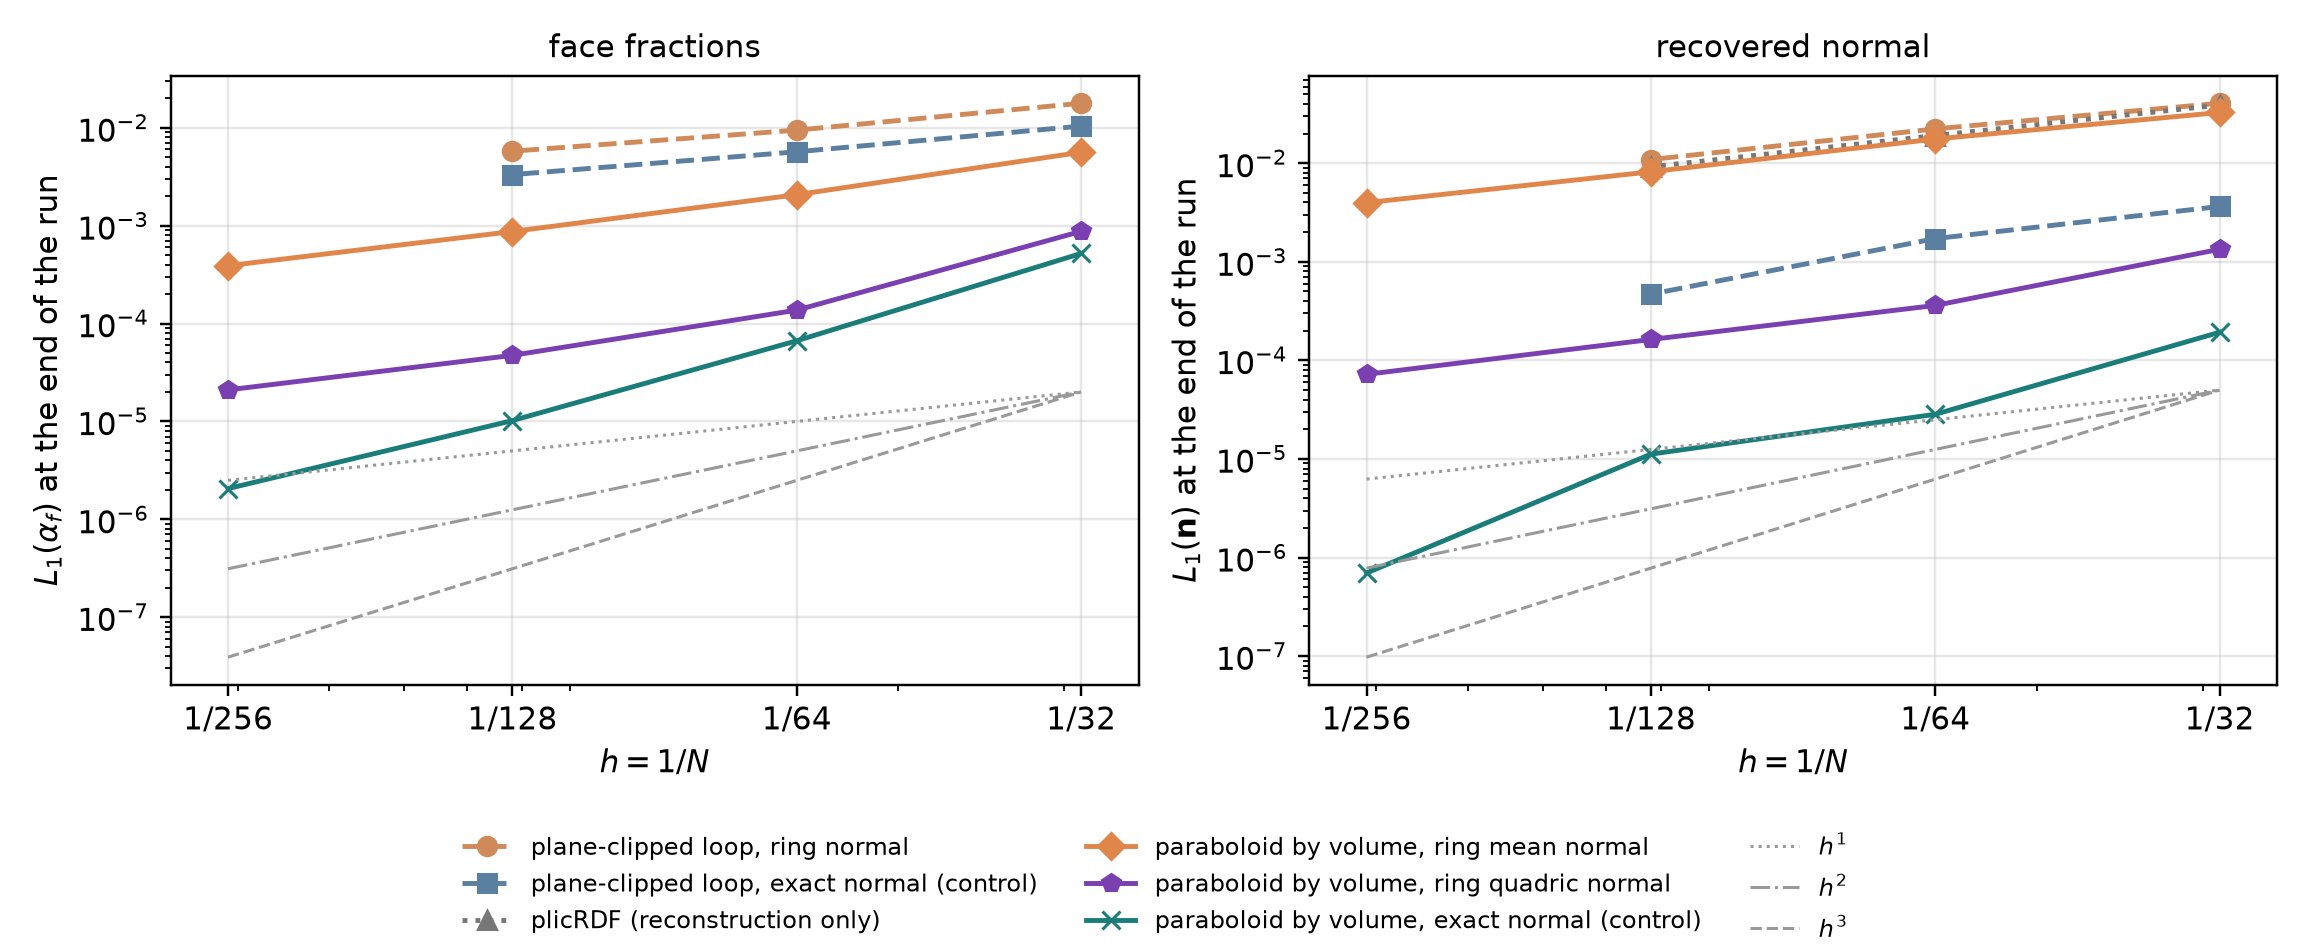
\includegraphics[width=\linewidth]{fig_ladders.png}
\caption{The resolution ladders of the translated sphere at $\mathrm{Co} = 0.2$: the face-fraction error (left) and the error of the normal recovered from the transported fractions (right) at the end of the run, against the cell size, for the plane-clipped loop (dashed; plicRDF's own normal dotted) and the dual advection with the ring-tensor paraboloid positioned by $\alpha_k$ (solid), $N = 32$ to $256$. The computed-normal rows of the paraboloid are first order on the finest pair at constants $18$ apart; the exact-normal control keeps order $2.3$ to $2.8$. Generated by \texttt{make\_fig\_ladders.py} from the exported order tables.}
\label{fig:tpf-ladders}
\end{figure}

\begin{table}[htbp]
\centering
\caption{The dual advection with one surface per cell on the translated sphere of \cref{tab:tpf-sphere}, from the exact-sphere initial state, $N = 32, 64, 128$, $\mathrm{Co} = 0.1, 0.2, 0.5$: the exact sphere as every cell's surface (the control; its three rows are the normal measured against the translated sphere: the exact one the loop uses, the one recovered from the transported fractions by \cref{eq:avof-normal}, and the ring normal) and the ring-tensor paraboloid positioned by $\alpha_k$ with its frame from the exact normal, from the ring normal, from the ring quadric's normal, from the cell's own normal with the ring normal below $0.1h^2$, and from the cell's own normal. Per row and Courant number: $L_1(\alpha_f)$ at the end of the run on the finest mesh with the least-squares order $p$ over the three meshes and the order $p_1$ of the error after the first step; the normal and centroid errors with their orders; the shape error; the minimum of $\alpha$ over the run; the run maximum of the surface defect ($L_1$ over the interface cells of $\alpha_k$ against the volume under the surface); the CPU time per step on the finest mesh with the per-step diagnostics on. Rows that abort list the steps for the three meshes. Table body generated by \texttt{make\_table\_advection.py}.}
\label{tab:tpf-curved}
\footnotesize
\setlength{\tabcolsep}{3pt}
\resizebox{\linewidth}{!}{% written by prepare_tables.py from table_advection_curved.tex -- do not edit
% Auto-generated by docs/davof/davof-article/make_table_advection.py -- do not edit.
\begin{tabular}{llrrrrrrrrrrr}
\toprule
surface, normal & Co & $L_1(\alpha_f)$ & $p$ & $p_1$ & $L_1(\mathbf{n})$ & $p$ & $L_1(\mathbf{x})$ & $p$ & $E_{\mathrm{shape}}$ & $\min_t \alpha$ & defect & s/step \\
\midrule
exact sphere, exact & 0.1 & 7.78e-13 & -- & -- & 1.07e-05 & 1.47 & 2.57e-05 & 1.98 & 2.30e-05 & -9.82e-15 & 9.28e-10 & 5.64 \\
 & 0.2 & 3.26e-13 & -- & -- & 1.07e-05 & 1.47 & 2.57e-05 & 1.98 & 2.30e-05 & -9.53e-15 & 2.98e-10 & 3.38 \\
 & 0.5 & 3.12e-15 & -- & -- & 1.07e-05 & 1.47 & 2.57e-05 & 1.98 & 2.30e-05 & -1.00e-14 & 3.32e-11 & 3.81 \\
\midrule
exact sphere, own & 0.1 & 7.78e-13 & -- & -- & 1.37e-04 & 1.40 & 2.57e-05 & 1.98 & 2.30e-05 & -9.82e-15 & 9.28e-10 & 5.61 \\
 & 0.2 & 3.26e-13 & -- & -- & 1.37e-04 & 1.40 & 2.57e-05 & 1.98 & 2.30e-05 & -9.53e-15 & 2.98e-10 & 5.69 \\
 & 0.5 & 3.12e-15 & -- & -- & 1.37e-04 & 1.40 & 2.57e-05 & 1.98 & 2.30e-05 & -1.00e-14 & 3.32e-11 & 6.36 \\
\midrule
exact sphere, ring & 0.1 & 7.78e-13 & -- & -- & 7.68e-03 & 0.98 & 2.57e-05 & 1.98 & 2.30e-05 & -9.82e-15 & 9.28e-10 & 5.60 \\
 & 0.2 & 3.26e-13 & -- & -- & 7.68e-03 & 0.98 & 2.57e-05 & 1.98 & 2.30e-05 & -9.53e-15 & 2.98e-10 & 5.84 \\
 & 0.5 & 3.12e-15 & -- & -- & 7.68e-03 & 0.98 & 2.57e-05 & 1.98 & 2.30e-05 & -1.00e-14 & 3.32e-11 & 3.72 \\
\midrule
ring-tensor paraboloid, exact & 0.1 & 1.10e-05 & 2.87 & 2.81 & 1.15e-05 & 2.10 & 2.57e-05 & 2.00 & 2.30e-05 & -8.51e-14 & 3.50e-16 & 3.83 \\
 & 0.2 & 1.02e-05 & 2.84 & 2.76 & 1.12e-05 & 2.05 & 2.57e-05 & 1.99 & 2.30e-05 & -7.12e-14 & 3.31e-16 & 4.47 \\
 & 0.5 & 1.11e-05 & 2.87 & 2.82 & 1.15e-05 & 2.31 & 2.57e-05 & 1.99 & 2.30e-05 & -2.00e-13 & 3.42e-16 & 4.94 \\
\midrule
ring-tensor paraboloid, ring & 0.1 & 8.52e-04 & 1.38 & 1.08 & 8.19e-03 & 1.00 & 2.89e-05 & 2.09 & 2.30e-05 & -3.73e-14 & 3.65e-16 & 4.30 \\
 & 0.2 & 8.71e-04 & 1.34 & 1.05 & 8.19e-03 & 1.00 & 2.85e-05 & 2.09 & 2.30e-05 & -5.07e-14 & 3.04e-16 & 4.35 \\
 & 0.5 & 1.22e-03 & 1.28 & 1.05 & 8.27e-03 & 0.99 & 2.83e-05 & 2.10 & 2.30e-05 & -1.62e-13 & 3.27e-16 & 4.91 \\
\midrule
ring-tensor paraboloid, ring quadric & 0.1 & 5.06e-05 & 2.24 & 1.88 & 1.67e-04 & 1.67 & 2.57e-05 & 2.00 & 2.30e-05 & -8.50e-14 & 3.52e-16 & 4.35 \\
 & 0.2 & 4.73e-05 & 2.11 & 1.92 & 1.63e-04 & 1.52 & 2.57e-05 & 2.00 & 2.30e-05 & -7.27e-14 & 3.31e-16 & 4.30 \\
 & 0.5 & 4.80e-05 & 1.93 & 2.23 & 1.61e-04 & 1.31 & 2.57e-05 & 1.99 & 2.30e-05 & -2.01e-13 & 3.42e-16 & 4.95 \\
\midrule
ring-tensor paraboloid, own, ring below $0.1h^2$ & 0.1 & \multicolumn{11}{l}{aborted at step 317 ($N=32$)/128 ($N=64$)/115 ($N=128$)} \\
 & 0.2 & \multicolumn{11}{l}{aborted at step 108 ($N=64$)/77 ($N=128$)} \\
 & 0.5 & \multicolumn{11}{l}{aborted at step 41 ($N=32$)/50 ($N=64$)/61 ($N=128$)} \\
\midrule
ring-tensor paraboloid, own & 0.1 & \multicolumn{11}{l}{aborted at step 66 ($N=32$)/76 ($N=64$)/82 ($N=128$)} \\
 & 0.2 & \multicolumn{11}{l}{aborted at step 46 ($N=32$)/63 ($N=64$)/68 ($N=128$)} \\
 & 0.5 & \multicolumn{11}{l}{aborted at step 45 ($N=32$)/51 ($N=64$)/54 ($N=128$)} \\
\bottomrule
\end{tabular}
}
\end{table}

\begin{table}[htbp]
\centering
\caption{The translated plane of \cref{tab:tpf-plane} with the ring-tensor paraboloid positioned by $\alpha_k$ and the dual advection, in the format of that table: per normal source and Courant number the number of the eight runs in which the face fractions and the normal stay at round-off over the whole run, and the run maximum of $L_1(\alpha_f)$ at $N = 160$ and $\mathrm{Co} = 0.5$ on the normal arm. Table body generated by \texttt{make\_table\_advection.py}.}
\label{tab:tpf-curved-plane}
\footnotesize
\setlength{\tabcolsep}{4pt}
\resizebox{0.8\linewidth}{!}{% written by prepare_tables.py from table_advection_curved_plane.tex -- do not edit
% Auto-generated by docs/davof/davof-article/make_table_advection.py -- do not edit.
\begin{tabular}{lrrr}
\toprule
surface, normal & Co $= 0.2$ & Co $= 0.5$ & $\max_t L_1(\alpha_f)$, $N = 160$, Co $= 0.5$ \\
\midrule
ring-tensor paraboloid, exact normal & 8/8 & 8/8 & 8.14e-14 \\
ring-tensor paraboloid, ring normal & 8/8 & 8/8 & 9.81e-14 \\
ring-tensor paraboloid, own normal & 1/8 & 0/8 & 1.18e-01 \\
\bottomrule
\end{tabular}
}
\end{table}

\begin{table}[htbp]
\centering
\caption{The fourth mesh: the ring-tensor paraboloid positioned by $\alpha_k$ at $N = 256$ ($33.6$ million cells, 96 processors, 1280 steps, $\mathrm{Co} = 0.2$; bounded and conservative, no fit fallback and no anchor failure) against $N = 128$, with the pairwise order. The exact-normal row's normal reading is the offset of the reference point, not an error (\ref{app:transport}), and is omitted. On 96 processors $7$ to $87$ of the $2\cdot10^5$ curved faces per step were left without a surface at processor corners, a gap of the parallel exchange absent in serial; against the serial digits at $N = 128$ its effect is $4\cdot10^{-5}$ to $6\cdot10^{-4}$ relative in the end values and $10^{-3}$ in the pairwise orders.}
\label{tab:tpf-n256}
\footnotesize
\begin{tabular}{llrrr}
\toprule
normal in the frame & error & $N = 128$ & $N = 256$ & order \\
\midrule
exact (control) & $L_1(\alpha_f)$ & 1.02e-05 & 2.06e-06 & 2.30 \\
 & $L_1(\mathbf{x})$ & 2.57e-05 & 6.27e-06 & 2.03 \\
ring quadric & $L_1(\alpha_f)$ & 4.73e-05 & 2.10e-05 & 1.17 \\
 & $L_1(\mathbf{n})$ & 1.63e-04 & 7.22e-05 & 1.18 \\
 & $L_1(\mathbf{x})$ & 2.57e-05 & 6.27e-06 & 2.03 \\
ring mean & $L_1(\alpha_f)$ & 8.71e-04 & 3.90e-04 & 1.16 \\
 & $L_1(\mathbf{n})$ & 8.19e-03 & 3.98e-03 & 1.04 \\
 & $L_1(\mathbf{x})$ & 2.85e-05 & 7.16e-06 & 1.99 \\
all rows & $E_{\mathrm{shape}}$ & 2.30e-05 & 5.74e-06 & 2.00 \\
\bottomrule
\end{tabular}
\end{table}

\subsection{Cost}
\label{sec:tpf-cost}

\Cref{tab:tpf-cost} compares the time per step with plicRDF on the same initial state, one core, $\mathrm{Co} = 0.2$, the error diagnostics reduced to the end of the run, three repetitions per case and the median taken; the three repetitions reproduce every error digit. The plane-clipped loop with the ring normal is cheaper than plicRDF, because its reconstruction is one sum of face fractions, one ring sum and one plane positioning per interface cell where plicRDF iterates its stencil ten times. The dual advection costs $1.2$ to $1.9$ times plicRDF after four changes to its first implementation, which had cost $3$ to $6$ times: planar faces integrated whole and only warped faces fanned, the diagnostics off unless asked for, the cell polyhedron built once per cell, and the volume anchor by the consecutive cubic spline positioning of \citet{Maric2021CCS} at $3.4$ volume evaluations per cell and step in place of $6.3$. The remaining difference is the Kromer--Bothe volume of every prism of the faces of the interface cells and their neighbours, where the plane loop has one plane cut per face.

\begin{table}[htbp]
\centering
\caption{Time per step on the translated sphere, one core, $\mathrm{Co} = 0.2$, medians of three repetitions with the diagnostics reduced to the end of the run (the node scatter of the medians is about $20\,\%$). The profile of one node: in the plane-clipped loop the DAVOF reconstruction takes $106\,\mathrm{s}$ of the $521\,\mathrm{s}$ advection time against $398$ of $811\,\mathrm{s}$ for plicRDF, the face update about $25\,\mathrm{s}$ more than plicRDF's flux; in the first implementation of the dual advection $57\,\%$ of the step was the volume anchor, $14\,\%$ two diagnostics of the anchor, $9\,\%$ the prism volumes, $7\,\%$ the face fractions, and the second-ring search, the ring normal and the tensor fit below $1\,\%$ each.}
\label{tab:tpf-cost}
\footnotesize
\begin{tabular}{lrrr}
\toprule
method & $N = 32$ & $N = 64$ & $N = 128$ \\
\midrule
plicRDF (plane-loop study) & $=$ DAVOF & $0.15\,\mathrm{s}$ & $1.72\,\mathrm{s}$ \\
plane-clipped loop, ring normal & $=$ plicRDF & $0.13\,\mathrm{s}$ & $1.31\,\mathrm{s}$ \\
\midrule
plicRDF (paraboloid study) & $0.031\,\mathrm{s}$ & $0.18\,\mathrm{s}$ & $1.8\,\mathrm{s}$ \\
paraboloid by volume, ring normal & $0.053\,\mathrm{s}$ ($1.7\times$) & $0.36\,\mathrm{s}$ ($1.9\times$) & $2.1\,\mathrm{s}$ ($1.2\times$) \\
same, first implementation & $6\times$ & $3.5\times$ & $3\times$ \\
\bottomrule
\end{tabular}
\end{table}

\subsection{Perturbed hexahedra}
\label{sec:tpf-perturbed}

The same two tests on hexahedra with every vertex displaced by up to $0.1h$ (warped faces, $\mathrm{Co} = 0.2$) measure what a scalar fraction per face cannot carry: on a warped face the wetted area vector is the transportable quantity (\cref{sec:warped}). \Cref{tab:tpf-perturbed} lists the outcome. With the scalar fraction no row passes the plane gate, and the exact-normal control shows that the defect is in what is stored per face, not in the normal; on the sphere every plane-clipped DAVOF row diverges, while plicRDF and isoAlpha stay bounded with normal errors that do not converge either, ten times their static values on the same meshes. With the wetted area vector per face, re-anchored centroids in the tensor fit and the flux prism fanned about the face centre, the translated plane stays at round-off in 11 of 12 runs with the exact and with the ring normal. On the perturbed sphere the dual advection completes without abort but is not bounded; the boundedness on perturbed meshes is the open item there, and distorted-mesh transport is an open question for the framework as a whole, not for DAVOF alone. The hexahedral results above are untouched by this.

\begin{table}[htbp]
\centering
\caption{Transport on hexahedra with every vertex displaced by up to $0.1h$, $\mathrm{Co} = 0.2$. The face state is either the scalar fraction $\alpha_f$ or the wetted area vector $\mathbf{a}_f = \sum_t A^{\mathrm{wet}}_t \mathbf{n}_t$ over the face's fan triangles (branch \texttt{davof-warped} of the fork; with re-anchored centroids in the tensor fit and the flux prism fanned about the face centre).}
\label{tab:tpf-perturbed}
\footnotesize
\begin{tabular}{p{0.2\linewidth}p{0.17\linewidth}p{0.55\linewidth}}
\toprule
test & face state & outcome \\
\midrule
plane, plane-clipped loop & scalar fraction & no row passes the gate; exact normal: the normal at round-off, the fractions off by $1$ to $5\,\%$; ring normal: the fraction error grows to $0.03$ to $0.11$ within the $0.2L$ travel \\
plane, dual advection & scalar fraction & ring normal at $2\cdot10^{-3}$, flat in $N$ \\
plane, dual advection & area vector & at round-off in 11 of 12 runs ($N = 20$, $40$, $80$, both arms, exact and ring normal); the twelfth, the ring row at $N = 80$ on the oblique arm, carries single-face jumps to $10^{-8}$ at four steps on faces a vertex of which grazes the plane \\
\midrule
sphere, plane-clipped loop & scalar fraction & every DAVOF row diverges, the exact-normal control included (stopped after 144 to 315 steps); plicRDF and isoAlpha bounded with converging shape errors and normal errors of $4.9\cdot10^{-2}$ to $8.8\cdot10^{-2}$ (plicRDF, $N = 32$ to $128$) that do not converge \\
sphere, dual advection & either & completes without abort, not bounded ($\min\alpha$ down to $-3\cdot10^{-3}$ at $N = 64$, the anchor failing in up to $1163$ cells over a run); centroid error $2$ to $2.3$ times the hexahedral value, shape error below it \\
\bottomrule
\end{tabular}
\end{table}

\subsection{What the transport studies say}
\label{sec:tpf-summary}

The closed loop needs a filtered normal. The cell-local normal is exact for a plane, but fed the fractions of several surfaces it turns by their mismatch times the neighbours' lever arms over its own patch area, with no restoring force, and amplifies round-off on the plane and the $O(h^2)$ mismatch of neighbouring surfaces on the sphere; the one-ring average divides the same mismatch by about $9h^2$ and contracts, at the price of the ring's mean normal. With it the plane-clipped loop is, as the clipping law predicts, a first-order method in the face fractions that matches plicRDF in position and shape, stays within $35\,\%$ of it in the normal and costs less. A second-order clipping inside the plane loop does not repair it, because the plane flux does not keep $\alpha_k$ the volume under the surface. With one surface per cell for the flux and the face update, the surface may take the normal from the cell's own faces and nothing else: the six-coefficient surface that interpolates them is unstable, and the ring-tensor surface positioned by the conserved $\alpha_k$ is stable, bounded and conservative at every resolution and Courant number, with face fractions of the order of the normal fed back and a per-step error that does not accumulate over the period. What limits the computed-normal loop is the normal: on the fourth mesh the ring quadric's normal, and the face fractions with it, fall to first order with a constant eighteen times below the ring mean's, so a second-order method needs a normal of proven second order on the transported state, which no one-ring construction measured here provides beyond $N = 128$. Transport on warped faces needs the face quantities of \cref{sec:warped} in the update, and with them the plane stays at round-off on perturbed hexahedra.
